\documentclass[essay]{fer}


\usepackage[ruled,vlined]{algorithm2e}
\usepackage{blindtext}
\usepackage{caption}
\usepackage{float}
\usepackage[bottom]{footmisc}
\usepackage{graphicx}
\usepackage{hyperref}

\SetAlgorithmName{}{}{}
\SetKw{Continue}{continue}
\SetKw{In}{in}
\SetKw{Null}{NULL}
\SetKw{True}{TRUE}
\SetKw{False}{FALSE}
\SetKw{Reverse}{REVERSE}
\SetKw{EmptySet}{EMPTY\_SET}

\makeatletter
\newcommand\footnoteref[1]{\protected@xdef\@thefnmark{\ref{#1}}\@footnotemark}
\makeatother

\renewcommand{\baselinestretch}{1}


%--- PODACI O RADU / THESIS INFORMATION ----------------------------------------

% Naslov na engleskom jeziku / Title in English
\title{Performance comparison of a Prefix Trie and a Patricia trie}

% Naslov na hrvatskom jeziku / Title in Croatian
%\naslov{Usporedba performansi prefiksnog stabla i Patricia stabla}

% Autor / Author
\author{Marko Šelendić}

% Mentor 
\mentor{dr. sc. Juraj Dončević}

% Datum rada na engleskom jeziku / Date in English
\date{January, 2025}

% Datum rada na hrvatskom jeziku / Date in Croatian
%\datum{siječanj, 2025.}

%-------------------------------------------------------------------------------


\begin{document}


% Naslovnica se automatski generira / Titlepage is automatically generated
\maketitle


% Sadržaj se automatski generira / Table of contents is automatically generated.
\tableofcontents
% Nemoj označiti broj ove stranice / Do not number this page
\thispagestyle{empty}


% Odovud započinje numeriranje stranica / Page numbering starts from here
\mainmatter


%--- SAŽETAK / ABSTRACT --------------------------------------------------------

% Sažetak na hrvatskom
%\begin{sazetak}
  %Unesite sažetak na hrvatskom.

  %\blindtext
%\end{sazetak}

%\begin{kljucnerijeci}
  %prva ključna riječ; druga ključna riječ; treća ključna riječ
%\end{kljucnerijeci}


%--- UVOD / INTRODUCTION -------------------------------------------------------
\chapter{Introduction}
\label{chptr:introduction}

\section{Strings}

Strings are one of the most fundamental data types in computer science. We all know they represent sequences of characters and are ubiquitous in all kinds of applications – from simple natural text processing to advanced algorithms in DNA sequence analysis. In essence, a string is an ordered collection of characters, where each character is typically chosen from a predefined set known as the alphabet. For example, the binary alphabet consists of the characters \{0, 1\}, while the English alphabet contains 26 characters from 'A' to 'Z'.
Each alphabet is defined by a function that maps each integer (up to some maximum integer) to a unique character. Since each integer has a unique byte representation in memory, the mapping function transitively gives this property to strings as well. These functions can usually be represented by a table, therefore being called mapping tables. Additional namings include "code page", "character set", and "character encoding". There are many popular and widely used mapping tables, like ASCII, Unicode (UTF-8, UTF-16) and ANSI table, and they all differ in size and the set of characters they contain. 

In this work, we will assume that we are using the ASCII table since it is the most simple one. For example, using the ASCII table, the string "hello" would be mapped to the sequence of hexadecimal numbers [ 0x68 0x65 0x6C 0x6C 0x6F ],
which will then be numerical representations of the bytes in memory where the string is stored.

One of the questions we could be asking ourselves now is how we could mark the end of a string. In the ASCII table there is a character for such purpose, and it is the NULL character or 0x00 hexadecimally. In the rest of this paper, we will represent the NULL character with the symbol '¤'. Another possible solution is to use the already existing strings to define some other strings as their substrings. We can achieve this by utilizing the SPL string representation, where each (sub)string can be defined by a tuple (s, p, l) = (pointer to the stored string, pointer to or index of the starting position of the substring in the stored string, length of the substring).

For example, let us say we have the string "hello there" stored somewhere in memory, and that our index counting starts from 0. Now we can do the following:
\begin{algorithm}[h]
$s$ $\gets$ "hello there"\;
\;
$ss1$ $\gets$ ($s$, 0, 4); \tcp{"hell"}
\;
$ss2$ $\gets$ ($s$, 7, 3); \tcp{"her"}
\end{algorithm}

The latter approach could prove useful in situations in which we have a very large number of strings, and many long ones, because then, we would not have to duplicate its prefixes as new strings but could instead just use those already existing long strings for defining their substrings.

\section{Tries}

As we just mentioned, in addition to storing individual strings in memory, it is often necessary to store a large number of strings, which we will refer to as a dataset.
One often also needs to do some operations on the dataset, such as inserting a new string, searching for a specific string,
searching for a range of strings matching a given prefix, or deleting a string.
In order to perform these operations efficiently, it is necessary to choose a suitable and appropriate data structure. Also, when one says "efficient", this could mean "time efficient" or "memory efficient", and as the famous no-free-lunch\cite{no_free_lunch_ref} rule says, there is usually no way of improving one without hurting the other in the process.

With that said, one of the commonly used data structures for storing strings is a trie. A trie, also known as a prefix tree, is a tree-like data structure that stores a dynamic set of strings.
There are several variations of the trie data structure, such as a standard or prefix trie, a hashed trie, a compressed trie (also called a radix trie or a Patricia trie), etc. We will now explain the prefix trie and the Patricia trie data structures more in detail.


\subsection{Prefix trie}
\label{sec:prefix_trie}

The root node of the Prefix trie represents an empty string, while other nodes represent a prefix of one or more strings, or the whole string if they lie at the end of some transition with the index '¤'.

Each trie node is characterized by its parent (or lack thereof) and its children. The children lie at the ends of the node's outgoing transitions, each indexed by a unique character in the mapping table. The transitions can also be called edges, and we will use both terms interchangeably.
The transitions represent the characters that can follow the prefix represented by the node.
Therefore, no two outgoing edges of a node can have the same character.

We can search for a string in the trie by starting at the root node and following the edges corresponding to the characters of the string.
After the last character of the string is reached, we check if there exists an additional transition for character '¤',
i.e. if there exists a child node at the end of it.
If there is such a transition, the trie does contain our string.

\begin{figure}[h]
  \label{fig:prefix_example}
  \centering
  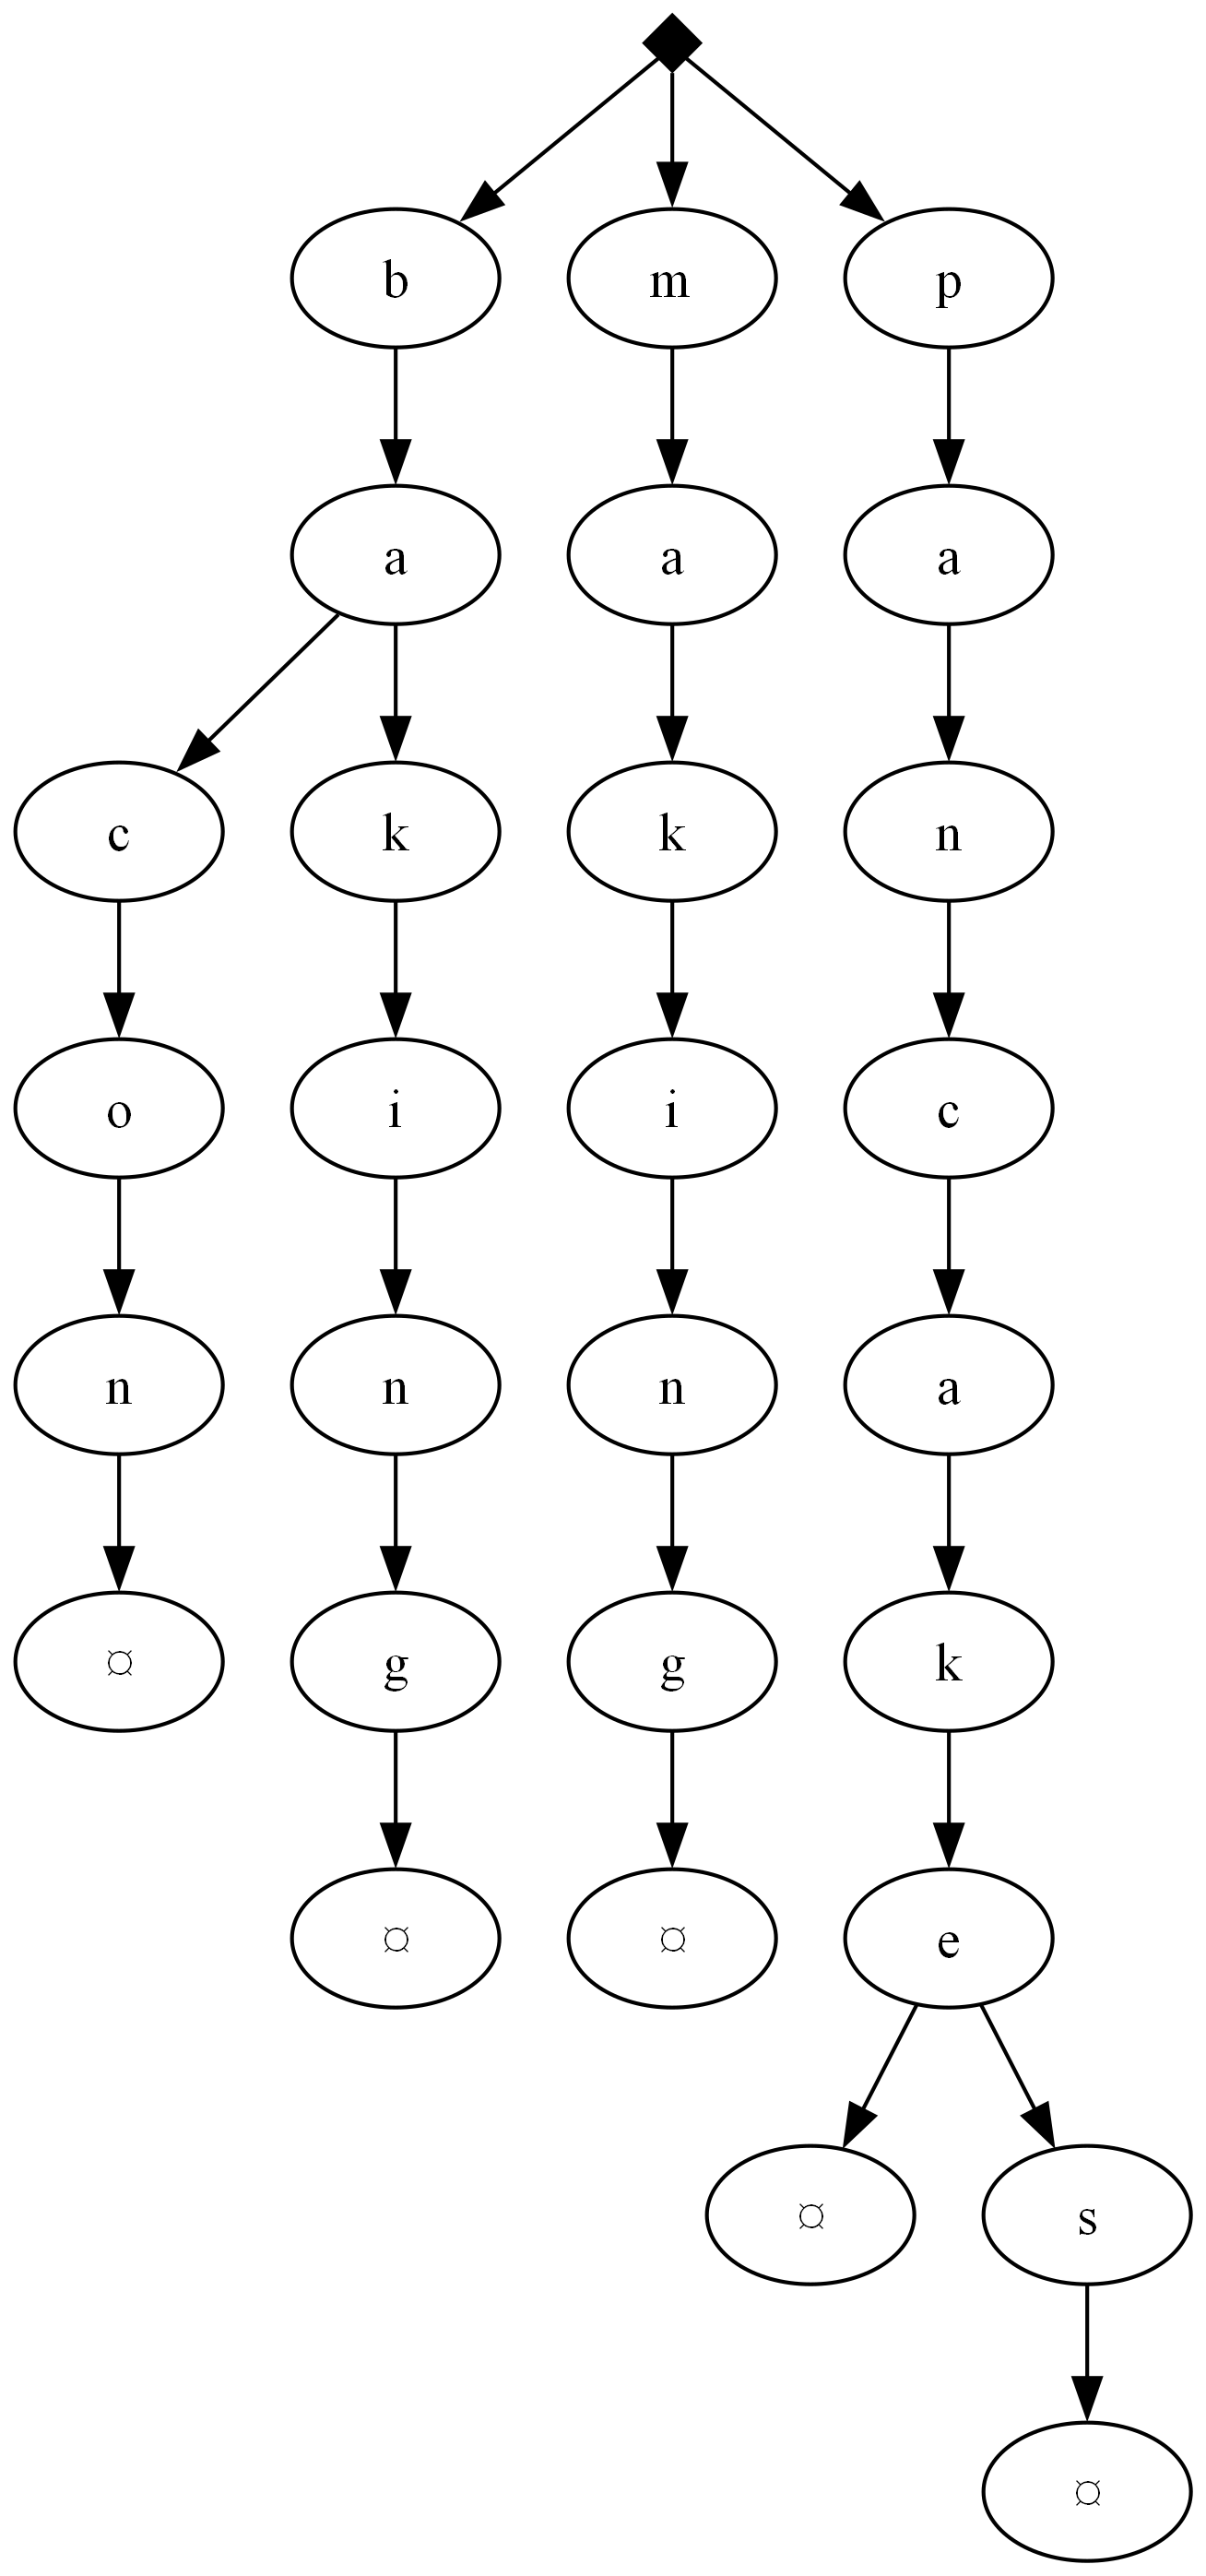
\includegraphics[width=0.32\textwidth]{Figures/prefix_trie_small_after_insertion.png}
  \caption{Prefix trie example after inserting strings: "baking", "pancakes", "making", "bacon", "pancake".}
\end{figure}


\subsection{Patricia trie}
\label{sec:patricia_trie}

As we can observe from the description of the Prefix trie, there are many nodes in the trie that have only one child and can therefore be seen as redundant.
The Patricia trie\cite{patricia_ref} (compressed trie, radix trie) attempts to solve this problem by merging the nodes with one single child.

Unlike the Prefix trie, while we are searching for a string in the Patricia trie, it is not enough to check if there exists a transition for the next character in the string. Instead, we have to check if the whole substring represented by a transition matches. If we can match only a part of it, then the trie does not contain the string we are searching for.

One way to more efficiently implement the Patricia trie is to utilize the aforementioned SPL string representation.
Now we do not have to create a new string for each prefix represented by a node, but can instead just use pointers to characters in strings that already exist in memory, represented by some other node at the end of some path that our node lies on.

\begin{figure}[h]
  \label{fig:patricia_example}
  \centering
  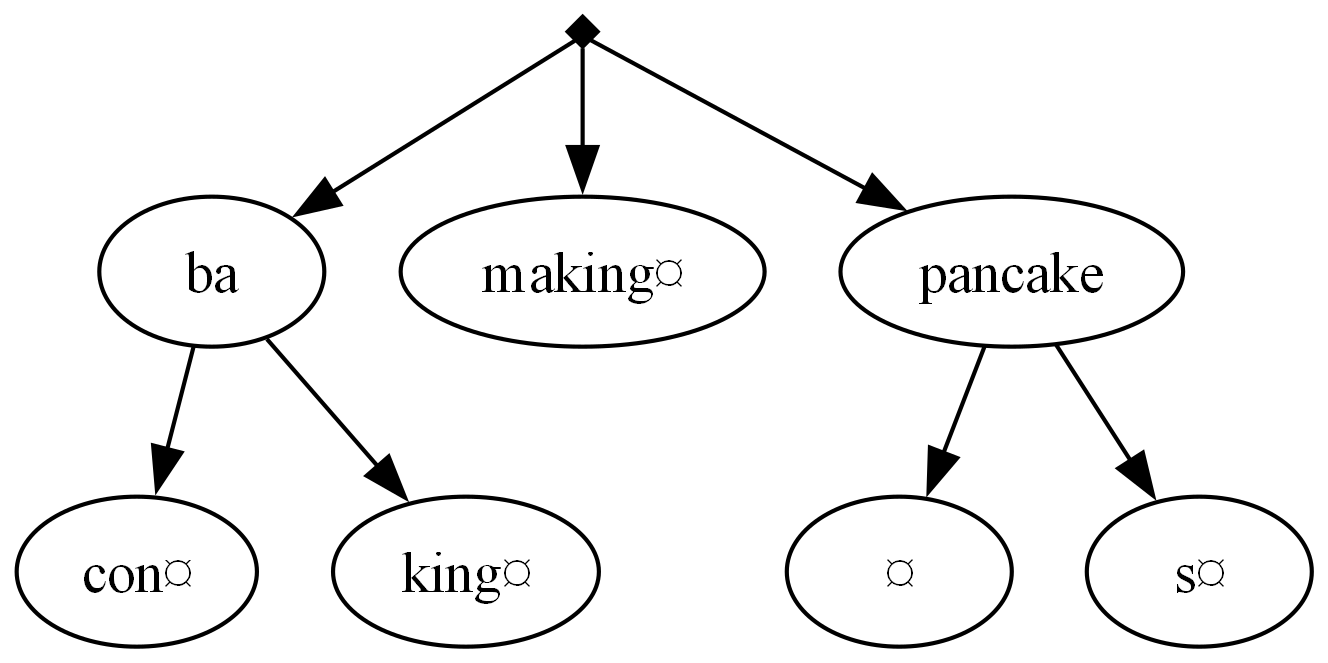
\includegraphics[width=0.85\textwidth]{Figures/patricia_trie_small_after_insertion.png}
  \caption{Patricia trie example after inserting strings: "baking", "pancakes", "making", "bacon", "pancake".}
\end{figure}

For example, in the figure above, let's say we have a string $s$ = "bacon¤" stored somewhere in memory. The "ba" node could then be represented by ($s$,0,2), while the "con¤" could be represented by ($s$,2,4). This way, the only strings we are effectively using are the ones that the trie is actually storing. We do not have to create new strings for our nodes that represent only some prefixes.

\subsection{Implementation specifics}
\label{sec:implementation_specifics}

To implement both tries a bit more efficiently, we will slightly modify the usual tree structure.

When we are doing a transition from one node to another, we want to avoid having to iterate through all the outgoing edges of the node to find the one we are looking for.
One way to achieve this would be to use a hash table, where the key would be the character of the transition and the value would be the pointer to the child node.
Another would be to use an array of pointers, where the index of the array would be the ASCII value of the character on the edge.

We will use the latter approach in our implementation. Each node will now have to store a pointer array of length 256 (the size of the ASCII table), with its elements initialized to NULL
(meaning that there are no transitions for any character from the node).
\footnote{Perhaps it is not obvious, but the Patricia trie can also utilize this approach.
No two transitions from a node can share the same prefix, therefore they also cannot have the same starting character.}
This way we are sacrificing the space complexity of our implementation in order to reduce the time complexity of the operations done on the trie.

In the rest of this paper, we will do a comparison of the two trie types, measuring their performance in typical operations, in terms of memory usage and time complexity.


%-------------------------------------------------------------------------------
\chapter{Algorithm presentation}
\label{chptr:algorithm_presentation}

We will now show the pseudocode for the insert, search, range search and delete operations for both the Prefix trie and the Patricia trie.
The actual implementation is written in Python and can be found in the GitHub repository\footnote[2]{\href{https://github.com/selendic/aads-seminar}{https://github.com/selendic/aads-seminar}}
along with the code for the experiments we conducted.
The implementations were heavily inspired by the ones found in the course lecture materials\cite{aads_ref}.


\section{Prefix trie operations}
\label{sec:prefix_trie_pseudocode}

\subsection{Insertion}

Insertion, as well as range search and deletion of a string into/from a Prefix trie, is in essence a search operation with extra steps. If the search operation ends in a success and returns an existing node, there is nothing else we need to do as the string is already in the trie. Otherwise, we go on to add a path of transitions and nodes below the returned one, one transition for each remaining non-matched character in the given string, and then an extra one for the terminating character '¤'.

\subsection{Search}

We already described the search operation in the introduction to tries. We start the search at the root node, and keep following the edges corresponding to the characters of the string. If at any point we find ourselves at a node with no outgoing transition to the next character in our string, the string does not exist in our trie.
After the last character of the string is reached, we do an additional check for a transition indexed by the character '¤'.
If there is such a transition, the trie does indeed contain our string.

\subsection{Range search}

We start the range search by doing a normal search, but without checking for the terminating character '¤' at the end of the operation.
If we get an existing node returned, we traverse its subtree (the one characterized by the node as its root), and return a set of all strings defined by the terminating nodes that we end up finding, i.e. the ones that lie on the other side of the transitions indexed by '¤', as those mark the ends of our stored strings.

\subsection{Deletion}

Again, we start the operation by doing a normal search without checking for '¤'.
If the search operation returns NULL, there is nothing to do as the given string does not exist in our trie.
Otherwise, we traverse the path we have just gone on backwards, and remove all nodes that remained as leaves, i.e. without children. In other words, we are removing a single branch that our string lied on.

\begin{figure}[H]
\centering

\begin{tabular}{cc}

\begin{minipage}[t]{0.47\textwidth}
  \scriptsize
  \begin{algorithm}[H]
  \caption{Insertion on a Prefix trie}
  \SetAlgoLined{}
  \KwIn{String $s$ to insert}
  \texttt{\\}
  current\_node $\gets$ root\;
  \ForEach{character $c$ \In $s$ + '¤'}{
      \If{current\_node has no child for $c$}{
          create new\_node\;
          add new\_node as a child of current\_node for $c$\;
      }
      current\_node $\gets$ child node for $c$\;
  }
  \end{algorithm}
\end{minipage}
&
\begin{minipage}[t]{0.47\textwidth}
  \scriptsize
  \begin{algorithm}[H]
  \caption{Search on a Prefix trie}
  \SetAlgoLined
  \KwIn{String $q$ to search for}
  \KwOut{Node in the trie corresponding to the input string, if it exists, else \Null}
  \texttt{\\}
  current\_node $\gets$ root\;
  \ForEach{character $c$ \In $q$ + '¤'}{
      \If{current\_node has no child for $c$}{
          \Return \Null\;
      }
      current\_node $\gets$ child node for $c$\;
  }
  \Return current\_node\;
  \end{algorithm}
\end{minipage} \\

\begin{minipage}[t]{0.47\textwidth}
  \renewcommand{\thempfootnote}{\arabic{mpfootnote}}
  \scriptsize
  \begin{algorithm}[H]
  \caption{Range search on a Prefix trie}
  \SetAlgoLined
  \KwIn{Prefix $q$ to search for}
  \KwOut{List or set of all strings that contain the given prefix}
  \texttt{\\}
  current\_node $\gets$ \texttt{Search}($q$)\footnoteref{search}\;
  \If{current\_node is \Null}{
      \Return \EmptySet\;
  }
  stack $\gets$ [(s, current\_node)]\;
  words $\gets$ \EmptySet\;
  \While{stack is not empty}{
      (current\_prefix, current\_node) $\gets$ stack.pop()\;
      \ForEach{child\_node of current\_node}{
      $c$ $\gets$ char for the transition to child\_node\;
          \If{$c$ == '¤'}{
              words.add(current\_prefix)\;
          }
          \Else{
              stack.push((current\_prefix + $c$, child\_node))\;
          }
      }
  }
  \Return words\;
  \end{algorithm}
\end{minipage}
&
\begin{minipage}[t]{0.47\textwidth}
  \renewcommand{\thempfootnote}{\arabic{mpfootnote}}
  \scriptsize
  \begin{algorithm}[H]
  \caption{Deletion on a Prefix trie}
  \SetAlgoLined{}
  \KwIn{String $s$ to remove}
  \KwOut{\True if the string was removed, \False if there was nothing to remove}
  \texttt{\\}
  end\_node$ \gets$ \texttt{Search}($s$)\footnoteref{search}\;
  \If{end\_node is \Null}{
      \Return \False\;
  }
  current\_node $\gets$ end\_node\;
  \ForEach{character $c$ \In \Reverse($s$ + '¤')}{
      \If{current\_node is not a leaf}{
          \textbf{break}\;
      }
      parent\_node $\gets$ current\_node.parent\;
      remove current\_node from the children of parent\_node\;
      current\_node $\gets$ parent\_node\;
  }
  \Return \True\;
  \end{algorithm}
  \footnotetext[3]{\label{search}Modified search so that it doesn't add the string-termination character ('¤') at the end of the input string}
\end{minipage}

\end{tabular}

\caption{Pseudocode for the operations in the Prefix Trie.}
\end{figure}


\section{Patricia Trie operations}
\label{sec:patricia_trie_pseudocode}

\subsection{Insertion}

Inserting into a Patricia trie is a bit more complicated. We start traversing it regularly, trying to match our string with the existing branches, and once we cannot do a full match on a transition anymore, there are two cases that can occur:
\begin{itemize}
    \item There is no match at all, meaning there is no transition defined for even the first remaining character of our string. This is the simpler case, as we can just take the rest of our string that remained unmatched, and insert a new node for it as its outgoing transition from the current node.
    \item We end up with a partial match. This means we have to split the node at the end of that particular transition, into two nodes: the parent node will keep the matched part of the transition and remain in the place of the current one, while the unmatched rest of the transition will go to its newly created child. In the end, we add a new child node to it, with the transition corresponding to the unmatched part of the string that we want to insert.
\end{itemize}

\subsection{Search}

The search operation is similar to its Prefix trie counterpart. We start by adding the '¤' at the end of our query string. While doing the search, unlike in the Prefix trie, now it is not enough to check if there exists a transition for the next character in the string. Instead, we have to check if the whole substring represented by a transition matches a part of the query string. If we can match only a part of it, then the trie does not contain the string we are searching for. Otherwise, we continue the traversal. Once we find ourselves at the end of some transition, and there are no more characters in our query string to match (we matched the whole string), then the string exists in the trie.

\subsection{Range search}

We start by doing a modified normal search, without the added character '¤', which will return whatever nodes it ends the search on, even in the case of empty and/or partial matches. Then, we return all the strings that we can end up with by continuing the traversal on the returned node's subtree, i.e. the subtree defined by the returned node as its root.

\subsection{Deletion}

The deletion operation should be simple. We do a normal search, and if we end up with a node returned, that node is the only one that we need to remove. Additionally, we need to do two checks. One is to see if the deleted node had exactly one sibling at the moment it was deleted, and if this is the case, then we need to merge it with their parent node. The need for the other check is the byproduct of our SPL string representation. If the deleted node had any siblings, we will traverse the search path vertically backwards, and replace the references to our deleted string in the nodes on the path with some other string referenced by one of the deleted node's siblings.

\begin{figure}[H]
\centering
\begin{tabular}{cc}

\begin{minipage}[t]{0.47\textwidth}
  \scriptsize
  \begin{algorithm}[H]
  \caption{Insertion on a Patricia trie}
  \SetAlgoLined{}
  \KwIn{String $s$ to insert}
  \texttt{\\}
  $s$ $\gets$ $s$ + '¤'\;
  $p$ $\gets$ 0\;
  $l$ $\gets$ length of $s$\;
  current\_node $\gets$ root\;
  \While{current\_node is root or is not a leaf}{
      child\_node $\gets$ child node for $s[p]$\;
      \If{child\_node is \Null}{
          \tcp{No match, insert the node}
          create new\_node with $s$[$p$ : $l$]\;
          current\_node.insert(new\_node)\;
          \Return new\_node\;
      }
      \If{we can match some remaining part of our string $s$ with a substring in child\_node}{
          \tcp{Full match, go deeper}
          $p$ $\gets$ $p$ + child\_node.l\;
          current\_node $\gets$ child\_node\;
          \Continue\;
      }
      \tcp{Partial match, split the node}
      $k$ $\gets$ length of matching substring\;
      create middle\_node with child\_node.$s$[child\_node.$p$ : child\_node.$p$+$k$]\;
      child\_node.p $\gets$ child\_node.p $+$ $k$\;
      child\_node.l $\gets$ child\_node.l $-$ $k$\;
      create end\_node with $s$[$p$+$k$ : $l$]\;
      put middle\_node in place of child\_node\;
      insert child\_node and end\_node as children of middle\_node\;
      \Return new\_node\;
  }
  \end{algorithm}
\end{minipage}
&
\begin{minipage}[t]{0.47\textwidth}
  \scriptsize
  \begin{algorithm}[H]
  \caption{Search on a Patricia trie}
  \SetAlgoLined
  \KwIn{String $q$ to search for}
  \KwOut{Node in the trie corresponding to the input string, if it exists, else \Null}
  \texttt{\\}
  $q$ $\gets$ $q$ + '¤'\;
  $p$ $\gets$ 0\;
  $l$ $\gets$ length of $q$\;
  current\_node $\gets$ root\;
  \While{current\_node is not a leaf and $p$ < $l$}{
      child\_node $\gets$ child node for $q$[$p$]\;
      \If{child\_node is \Null}{
          \Return \Null\;
      }
      \If{substring of child\_node does not match q[p : p+child\_node.l]}{
          \Return \Null\;
      }
      $p$ $\gets$ $p$ + child\_node.l\;
      current\_node $\gets$ child\_node\;
  }
  \Return current\_node if $p$ == $l$ else \Null\;
  \end{algorithm}
\end{minipage}

\end{tabular}
\caption{Pseudocode for Insert and Search operations in the Patricia Trie.}
\end{figure}


\begin{figure}[H]
\centering
\begin{tabular}{cc}

\begin{minipage}[t]{0.47\textwidth}
  \scriptsize
  \begin{algorithm}[H]
  \caption{Range search on a Patricia trie}
  \SetAlgoLined
  \KwIn{Prefix $q$ to search for}
  \KwOut{List or set of all strings that contain the given prefix}
  \texttt{\\}
  $p$ $\gets$ 0\;
  $l$ $\gets$ length of $q$\;
  current\_node $\gets$ root\;
  \While{current\_node is not a leaf and $p$ < $l$}{
      child\_node $\gets$ child node for $q$[$p$]\;
      \If{child\_node is \Null}{
          \Return \EmptySet\;
      }
      prefix\_len $\gets$ min(child\_node.l, $l$ - $p$)\;
      \If{$q$[$p$ : $p$+prefix\_len] != child\_node.s[child\_node.p : child\_node.p+prefix\_len]}{
          \Return \EmptySet\;
      }
      p $\gets$ p + prefix\_len\;
      current\_node $\gets$ child\_node\;
  }
  results $\gets$ \EmptySet\;
  stack $\gets$ [current\_node]\;
  \While{stack is not empty}{
      current\_node $\gets$ stack.pop()\;
      \If{current\_node is a leaf}{
          results.add(current\_node.s)\;
      }
      stack.push(children of current\_node)\;
  }
  \Return results\;
  \end{algorithm}
\end{minipage}
&
\begin{minipage}[t]{0.47\textwidth}
  \scriptsize
  \begin{algorithm}[H]
  \caption{Deletion on a Patricia trie}
  \SetAlgoLined{}
  \KwIn{String $s$ to remove}
  \KwOut{\True if the string was removed, \False if there was nothing to remove}
  \texttt{\\}
  final\_node $\gets$ \texttt{Search}(s)\;
  \If{final\_node is \Null}{
      \Return \False\;
  }
  current\_node $\gets$ final\_node.parent\;
  \If{current\_node is \Null}{
      \Return \False\;
  }
  current\_node.remove(final\_node)\;
  first\_child $\gets$ first child of current\_node if there is one\;
  is\_only\_child $\gets$ current\_node.num\_children == 1\;
  \If{is\_only\_child and current\_node.parent is not \Null}{
      merge first\_child with current\_node.parent\;
  }
  \If{first\_child is not \Null}{
      \tcp{Replace the references to the deleted string across all nodes in the chain with some other viable one}
      current\_node $\gets$ first\_child\;
      \While{current\_node.parent is not \Null}{
          \If{current\_node.parent.s == final\_node.s}{
              current\_node.parent.s = current\_node.s\;
          }
          current\_node $\gets$ current\_node.parent\;
      }
  }
  \Return \True\;
  \end{algorithm}
\end{minipage}

\end{tabular}
\caption{Pseudocode for Range Search and Delete operations in the Patricia Trie.}
\end{figure}

%-------------------------------------------------------------------------------
\chapter{Experiment setup}
\label{chptr:experiment_setup}

As for the experiments themselves, we used the google-10000-english-usa-no-swears\footnote[4]{\href{https://github.com/first20hours/google-10000-english}{https://github.com/first20hours/google-10000-english}} dataset, which contains the 10,000 most common English words, without swears.
To see the dependence of the performance on the size of the dataset,
the length of the subset of words used will start at 500 and increase by 500 until all 10,000 are used.
We did not filter the words by length. For each subset, we loaded them in the order they appeared in the dataset, so the results should be reproducible.

We measured the performance of the trie on the operations in the following way, repeated for each subset size:
\begin{itemize}
  \item Insertion was measured by inserting all the words from the subset into the trie.
  \item Search was then measured by searching for all the words in the trie.
  \item For range search, we decided to use all possible one- and two-character combinations from the lowercase English alphabet as prefixes:
        [a-z] + [a-z]×[a-z] = \{a, b, ..., z, aa, ab, ac, ..., yz, zz\}
  \item Deletion was measured by deleting all the words from the subset from the trie.
\end{itemize}

For each of these procedures, we measured the time it took to complete it and the peak memory consumption during the procedure.
We utilized the \texttt{time} and \texttt{tracemalloc} Python modules for this, due to both of them being simple to use and convenient for visualizing the results via \texttt{matplotlib}.
Memory consumption was additionally checked by utilizing the \texttt{cProfile} module to confirm that it aligns with the \texttt{tracemalloc} measurements, since the latter produces some level of overhead. However, we are doing a comparison, so this does not make a difference.


%-------------------------------------------------------------------------------
\chapter{Experiment results}
\label{chptr:experiment_results}

\section{Time performance comparisons}

\begin{figure}[H]
  \centering
  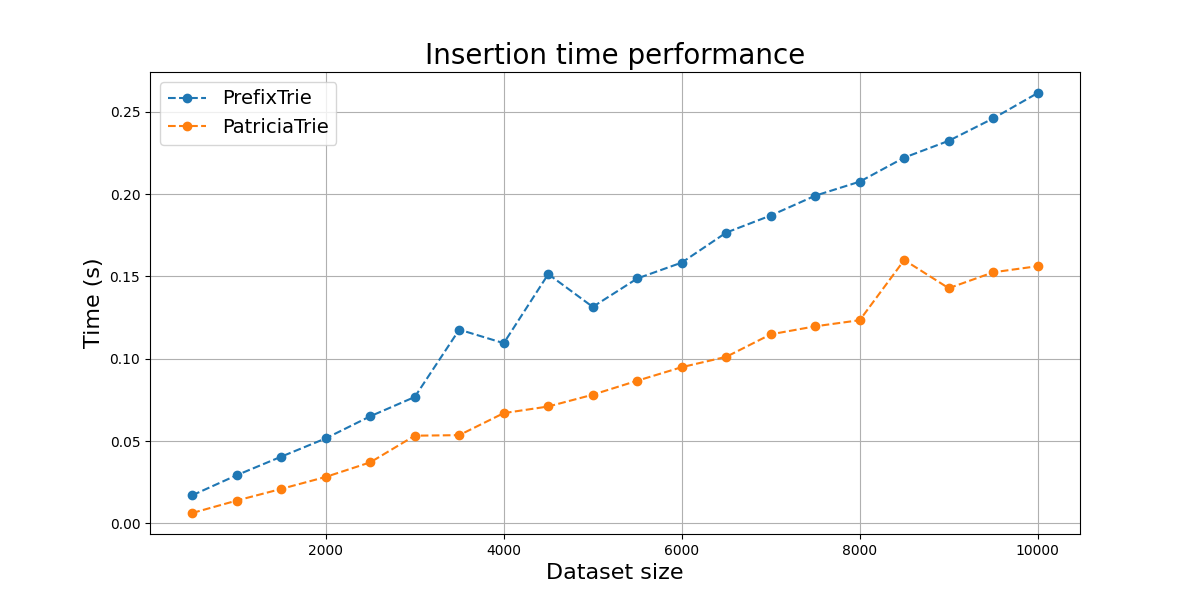
\includegraphics[width=0.95\textwidth]{Figures/insertion_time_performance.png}
  \caption{Insertion time performance comparison.}
  \label{fig:insertion_time}
\end{figure}

\begin{figure}[H]
  \centering
  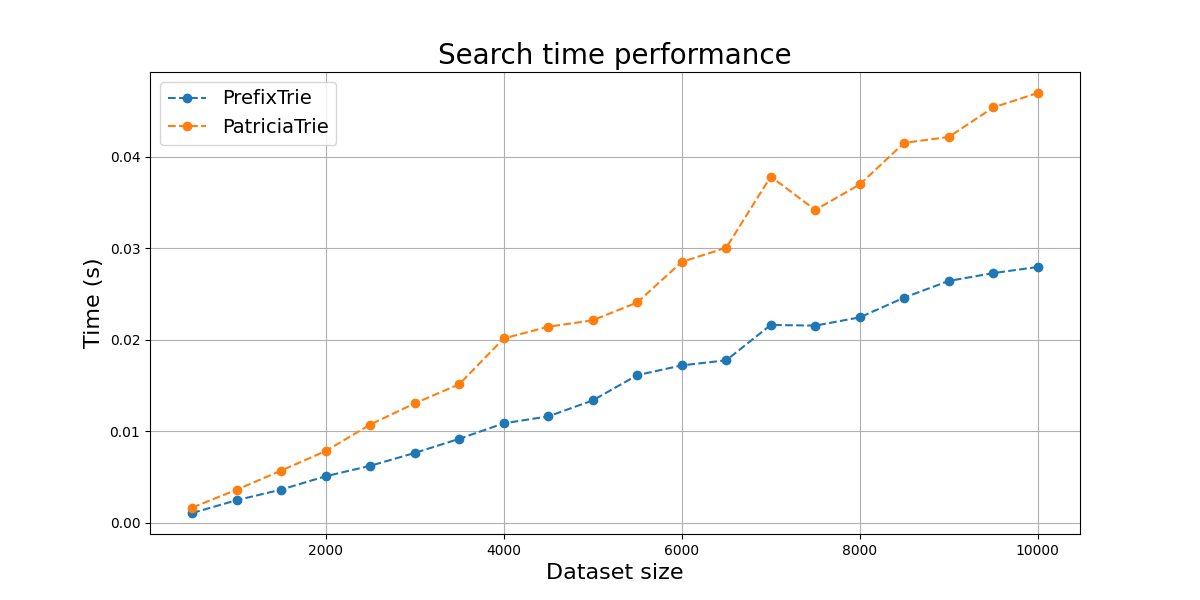
\includegraphics[width=0.95\textwidth]{Figures/search_time_performance.png}
  \caption{Search time performance comparison.}
  \label{fig:search_time}
\end{figure}

\begin{figure}[H]
  \centering
  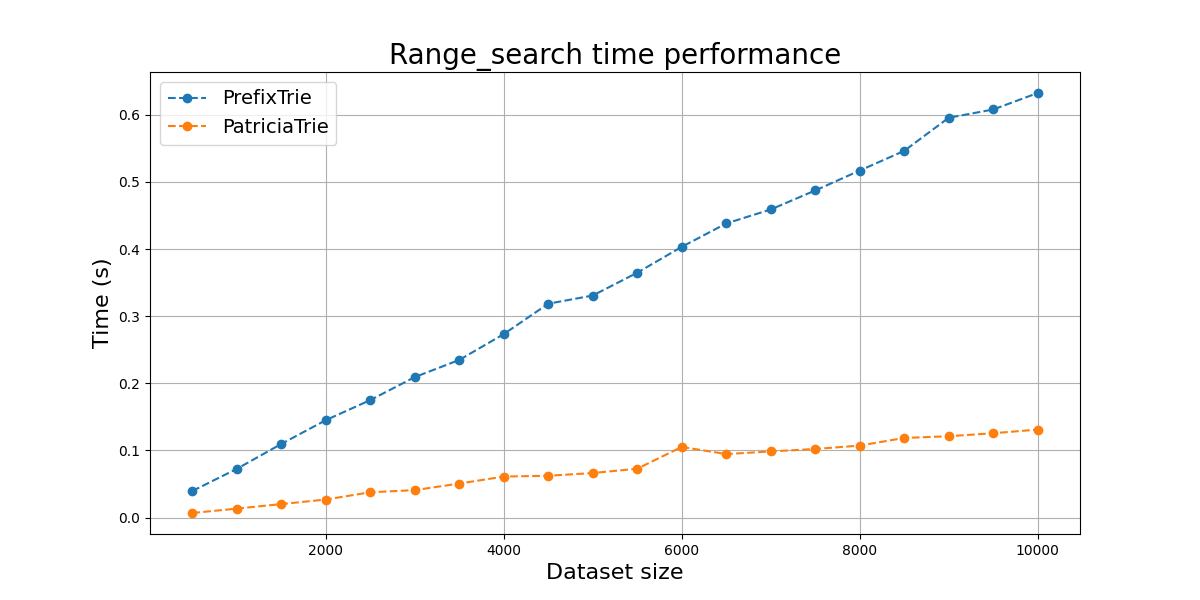
\includegraphics[width=1.00\textwidth]{Figures/range_search_time_performance.png}
  \caption{Range search time performance comparison.}
  \label{fig:range_search_time}
\end{figure}

\begin{figure}[H]
  \centering
  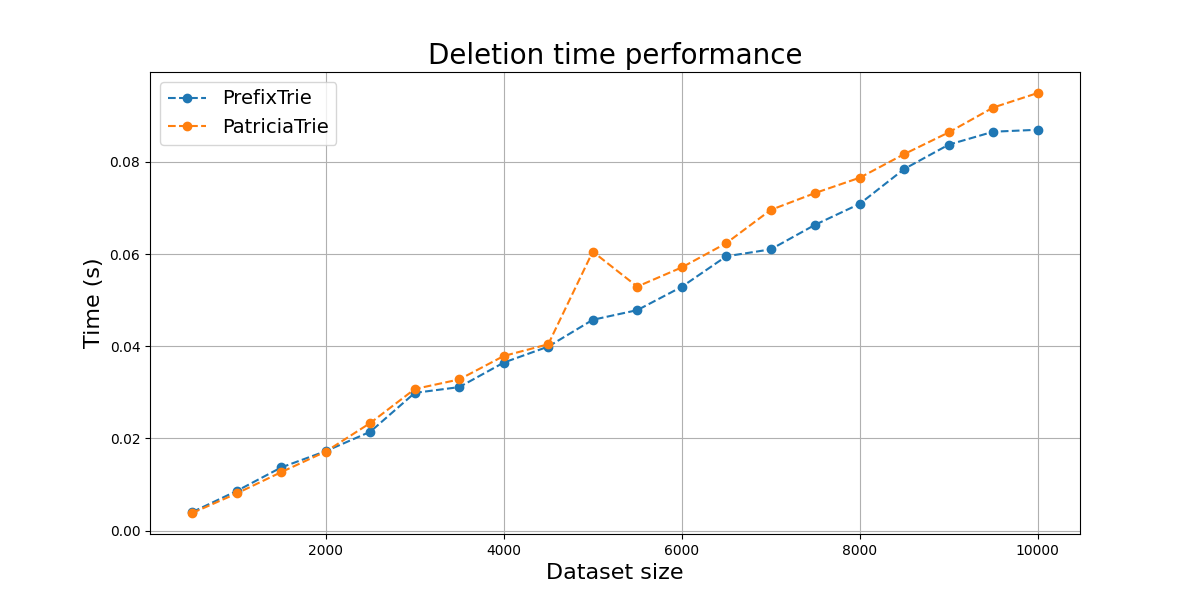
\includegraphics[width=1.00\textwidth]{Figures/deletion_time_performance.png}
  \caption{Deletion time performance comparison.}
  \label{fig:deletion_time}
\end{figure}


\section{Memory performance comparisons}

\begin{figure}[H]
  \centering
  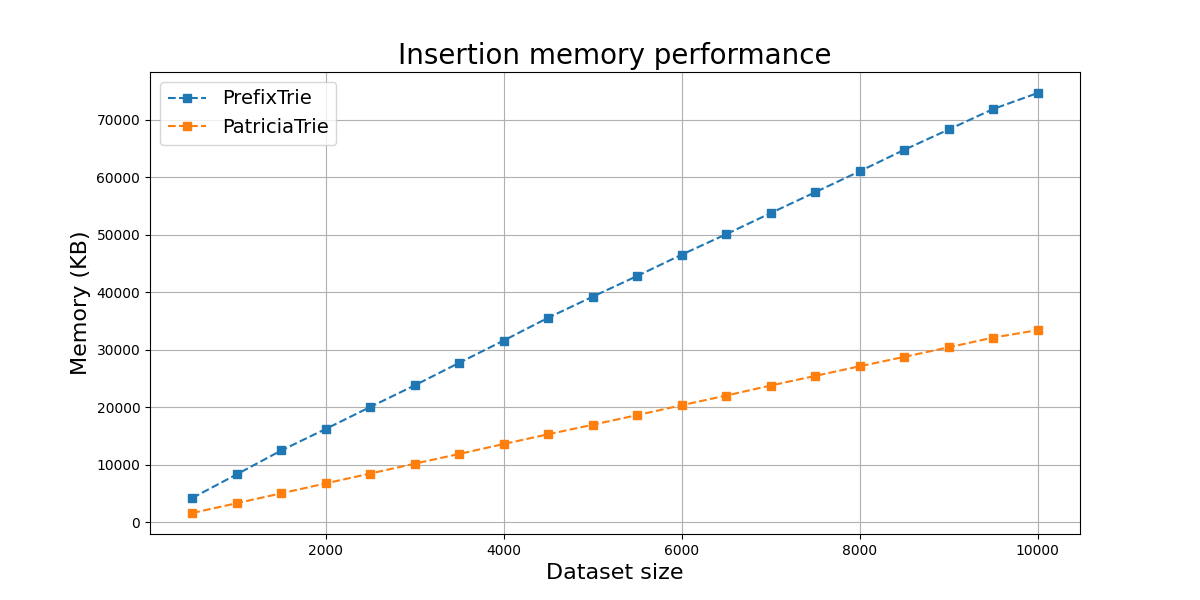
\includegraphics[width=1.00\textwidth]{Figures/insertion_memory_performance.png}
  \caption{Insertion memory performance comparison.}
  \label{fig:insertion_memory}
\end{figure}

\begin{figure}[H]
  \centering
  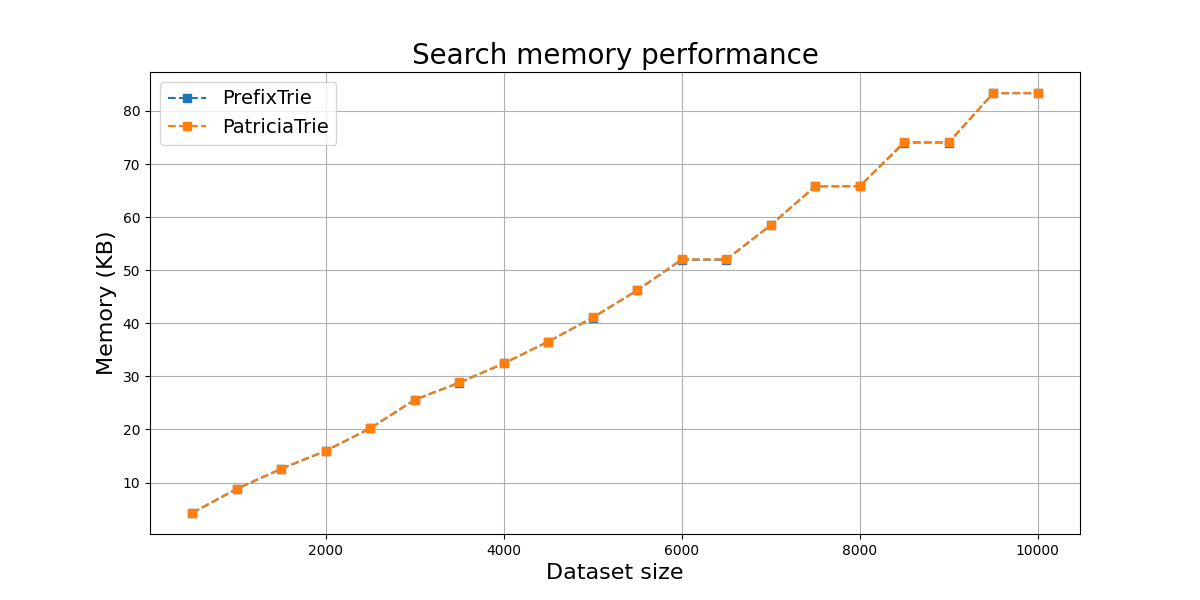
\includegraphics[width=1.00\textwidth]{Figures/search_memory_performance.png}
  \caption{Search memory performance comparison.}
  \label{fig:search_memory}
\end{figure}

\begin{figure}[H]
  \centering
  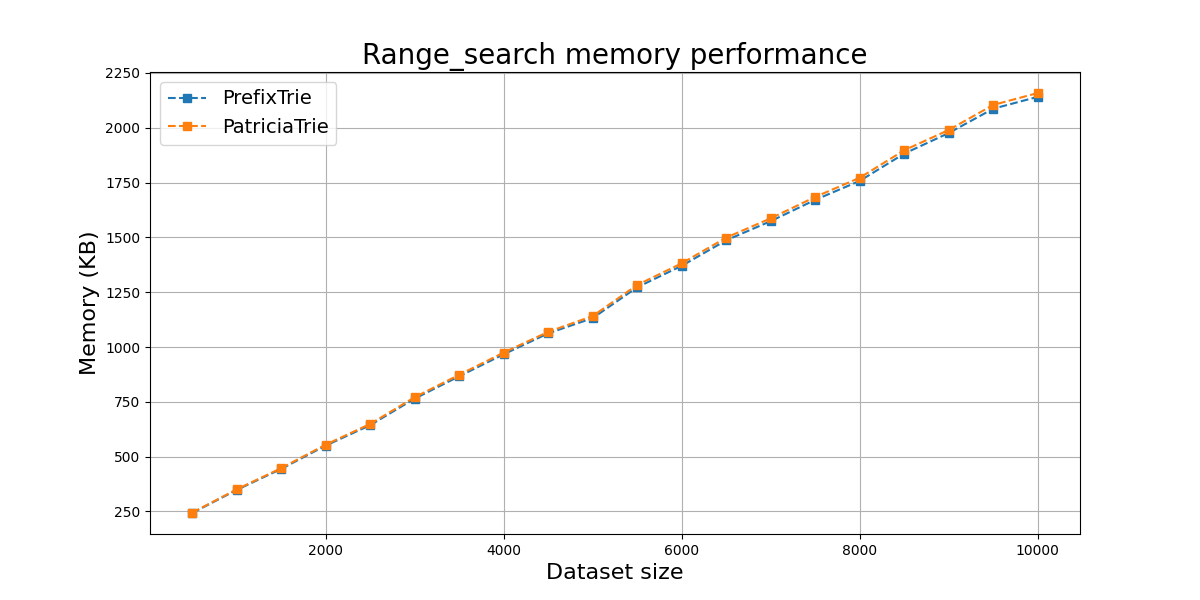
\includegraphics[width=1.00\textwidth]{Figures/range_search_memory_performance.png}
  \caption{Range search memory performance comparison.}
  \label{fig:range_search_memory}
\end{figure}

\begin{figure}[H]
  \centering
  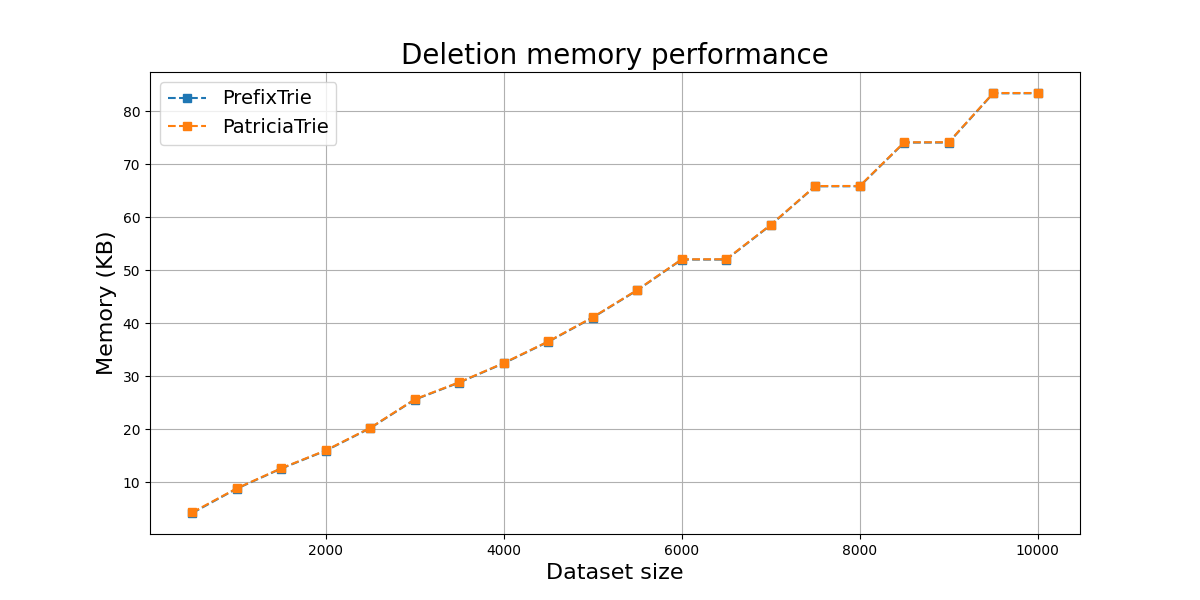
\includegraphics[width=1.00\textwidth]{Figures/deletion_memory_performance.png}
  \caption{Deletion memory performance comparison.}
  \label{fig:deletion_memory}
\end{figure}


%--- ZAKLJUČAK / CONCLUSION ----------------------------------------------------
\chapter{Discussion and conclusion}
\label{chptr:discussion_and_conclusion}

\section{Time performance}
\label{sec:time_performance_discussion}

The time performance results turned out as expected, for the most part.
The Patricia trie turned out to be a clear winner in insert and range search operations.
This is because in both of those cases, once it finds the matching node with the correct substring (or the lack thereof),
it can do the rest of the operation much quicker than the Prefix trie: insert at max two nodes in case of insertion,
and reach and return the strings contained at the leaves of the subtree in case of range search.
The Prefix trie on the other hand needs to insert a new node for each remaining character of the string,
and needs to traverse a lot more nodes after it matches the given prefix in case of range search.

The range operation favors the Patricia tree even more in our case, since in our experiments we are searching for very short prefixes, reducing the number of matches it needs to do even more. It would be interesting to see whether things would change if we introduced longer prefixes for the range search experiment.

As for the (exact) search operation, the Patricia trie actually turned out to be slower than the Prefix trie.
This does make sense after giving it some thought after all, because even though the Patricia trie usually contains fewer nodes,
it still needs to check the whole substring of the node to see if it matches the searched string, while traversing the Prefix trie is straight forward, and due to our array-of-pointers implementation, done in constant time.

The delete operation though seems to be an interesting case.
The difference is barely noticeable, and the winner varies from subset to subset, but also from run to run.
Let us try to explain why this is the case either way.
\begin{itemize}
  \item The first part of the deletion operation is the same for both tries: find the node that represents the string, which is done by calling the search operation,
        and we just showed that this is the only operation where the Prefix trie excels.
  \item The second part of the deletion operation differs between the two tries:
        \begin{itemize}
          \item The Prefix trie then has to go through the whole string in reverse and remove the nodes and edges that are no longer needed.
          \item The Patricia trie, on the other hand, only has to delete this one node that was found,
                and then check if there remained only one child node in the parent node of the deleted node and merge them if that is the case.
                In the end, it has to climb back the search path, and in each parent node that still has the deleted string stored, replace it with a string stored in one of the remaining child nodes.
        \end{itemize}
\end{itemize}
The results therefore seem to suggest that, for the Patricia trie, either the situation where only one child remains after the deletion operation is very rare,
or that its second part of the delete operation is much more quickly done.
If the latter turned out to be the case, we would have to conclude that indeed, in almost all situations,
there seem to be much fewer nodes in an average search path of the Patricia trie than in one of the Prefix trie.

Also, let us address the random spikes that can be noticed, for example while looking at the Patricia trie's search time performance at 7000 words and its deletion time performance at 5000 words. Sometimes they would show up on completely different places, and sometimes not show at all. Therefore, we are quite sure that we can safely ascribe them to the imperfections of the device that the tests were running on, but it would be a good idea to test this hypothesis by running the experiments on a few different devices.


\section{Memory consumption}
\label{sec:memory_consumption_discussion}

Memory performance results are a less interesting case, since everything turned out as expected.
The difference only manifests itself in the insertion operation,
since the only important factor is how the whole trie is stored, and the overhead of each operation is negligible.
The Patricia trie is the clear winner in this case, since it has to store a fewer number of nodes.
Indeed, despite the fact that there is more information needed to be stored in each node of the Patricia trie compared to the Prefix trie (due to the SPL string representation),
since we opted for the array-of-pointers approach in our implementation of transition/edge storage in both trie types,
the number of stored nodes ends up being a much more important factor when analyzing their memory consumption, largely outweighing the former one.


\section{Conclusion}
\label{sec:conclusion}

In conclusion, the Patricia trie is the clear winner in terms of memory consumption and time performance in most of the operations.
The only operation where this is not the case is the search operation, and even then
if we look at the specific amounts of time it took to complete the operation (the y-axis values on the search time performance graph),
rather than their differences, we can see that for both tries the time it took to complete the operation is extremely small.
Moreover, it is much smaller than the time it took to complete the other operations, so the difference in performance should also be of less significance to us than in other operations.

Therefore, if we would be specifically and only interested in the fastest retrieval of the exact strings stored in the trie,
and not care about the memory consumption or the speed of other operations such as insertion and range search at all,
we would opt for the Prefix trie.
In all other cases, the Patricia trie is clearly the better choice.


%--- LITERATURA / REFERENCES ---------------------------------------------------

% Literatura se automatski generira / References are automatically generated
% Upiši ime BibTeX datoteke bez .bib nastavka / Enter the name of the BibTeX file without .bib extension
\bibliography{references}


%--- PRIVITCI / APPENDIX -------------------------------------------------------

\backmatter{}

\end{document}
